\documentclass[a4paper,10pt]{report}
\usepackage[english]{babel}
\usepackage[utf8]{inputenc}
\usepackage{listings}
\usepackage{enumitem}
\usepackage{graphicx}

\graphicspath{{./figures}}


\title{A-FMM User Guide}
\author{Marco Passoni}
\date{}

\begin{document}

\maketitle


\chapter{Algorithm} 
In this chapter the theory behind this implementation of Aperiodic-Fourier Modal Method is discussed. The discussion is divided into three parts. The first part describes the theory behind the resolution of the Maxwell equation in the single 2D layer by expansion on Fourier basis. The second part explains the theory behind the scattering matrix algorithm, which links together the solutions of Maxwell equation of each 2D layer to get the solution for the complete structure. Both these parts follow the formulation developed by Lifeng Li for application of Fourier methods to crossed gratings, with very little modification. The third part describes the real and complex coordinate Fourier transform which allow the treatment of aperiodic structures with Fourier modal methods, following the work of P. Lalanne and J. P. Hugonin. In all the following treatment we will assume plane $xy$ as the plane in which the 2D periodic layer extends, and $z$ direction the stacking direction. Field Vector will be indicated with Bold $\mathbf{F}$. Italic $E$ will indicate both field components and vectors of the Fourier coefficient of the corresponding fields, specifying it when necessary. 

\section{Maxwell equation in 2D layers: the eigenvalue problem} \label{sec:eigenploblem}
The aim of this section is to describe the theory behind the solution of the Maxwell equation in a single 2D layer which could be patterned in a periodic way. Leaning on the periodicity of the structure is it possible to expand an arbitrary component of the field $\mathbf{F}$ in pseudo-fourier basis:
\begin{equation} \label{eq_Fourier_exp}
F_\sigma = \sum_\mathbf{k}F_\sigma^{(\mathbf{k})}(z)\exp{i(k_xx+k_yy)}
\end{equation} 
where $\mathbf(k)=\mathbf{k}_0 + \mathbf{K}$ wavevector of the pseudo Fourier expansion, composed by the the in plane wavevector $\mathbf{k}_0$ plus any vector $\mathbf{K}$ of the reciprocal lattice. The $z$ dependence of the coefficients of the expansion has to be calculated from Maxwell equations which, when expanding the components, take the form:
\begin{equation} \label{eq:Maxwell}
\left\{\begin{array}{c}
\partial_y E_z - \partial_z E_y = ik_0 \mu H_x \\
\partial_z E_x - \partial_x E_z = ik_0 \mu H_y \\
\partial_x E_y - \partial_y E_x = ik_0 \mu H_z \\
\end{array} \right.
\qquad
\left\{\begin{array}{c}
\partial_y H_z - \partial_z H_y = -ik_0 \varepsilon E_x \\
\partial_z H_x - \partial_x H_z = -ik_0 \varepsilon E_y \\
\partial_x H_y - \partial_y H_x = -ik_0 \varepsilon E_z \\
\end{array} \right.
\end{equation}  
where $k_0,\mu,\varepsilon$ are respectively the wavevector in vacuum of the radiation ($\omega/c$), magnetic permeability and the dielectric constant. From now on we will make the assumption of non magnetic ($\mu=1$), linear and isotropic material (although generalization to anisotropic material with principal axis coincident with the reference axis will be discussed later).
At this point we can write equation \ref{eq:Maxwell} in Fourier space, being careful to employ the right factorization rule when concurrent jumps in the function involved are present. After doing this we can recast the Maxwell equation in matrix form involving only the in-plane components of the fields in the following manner:
\begin{equation} \label{eq:def_F}
-\frac{i}{k_0} \partial_z \left[ \begin{array}{c} E_x \\ E_y \end{array} \right] =
\left[ \begin{array}{cc} K_x \hat{\varepsilon}^{-1} K_y & I - K_x \hat{\varepsilon}^{-1} K_x \\ K_y \hat{\varepsilon}^{-1} K_y - I & -K_y \hat{\varepsilon}^{-1} K_x \end{array} \right]
\left[ \begin{array}{c} H_x \\ H_y \end{array} \right] =
F \left[ \begin{array}{c} H_x \\ H_y \end{array} \right]
\end{equation}

\begin{equation} \label{eq:def_G}
-\frac{i}{k_0} \partial_z \left[ \begin{array}{c} H_x \\ H_y \end{array} \right] =
\left[ \begin{array}{cc} -K_xK_y & K_x^2 - \hat{\varepsilon}_{y,x} \\ \hat{\varepsilon}_{x,y} - K_y^2 & K_yK_x \end{array} \right]
\left[ \begin{array}{c} E_x \\ E_y \end{array} \right]= 
G \left[ \begin{array}{c} E_x \\ E_y \end{array} \right]
\end{equation}
Here a little of explanation on the notation is needed. First, $E_x,E_y,H_x,H_y$ are the vector of the Fourier coefficient of the Fourier components. If the expansion is truncated with $N$ reciprocal lattice vector, these vector has dimension $N$. All the others terms are $N \times N$ matrices composed as follow. The matrix $K_x$ is a diagonal matrix composed with the $x$ component of the wavevector of the expansion $K_x(\mathbf{k},\mathbf{k}') = k_x \delta_{\mathbf{k}\mathbf{k}'}$, and similar for $K_y$. $I$ is the $N \times N$ identity matrix.  The matrix $\hat{\varepsilon}$ is a Toeplitz matrix composed with the Fourier transform of the dielectric constant:
\begin{equation}
\hat{\varepsilon}(\mathbf{k},\mathbf{k}') = \frac{1}{A_c} \int_{A_c} \varepsilon(x,y)\exp(-i[(k_x-k_x')x+(k_y-k_y')y]) dxdy
\end{equation}
The other two matrices, $\hat{\varepsilon}_{x,y}$ and $\hat{\varepsilon}_{x,y}$ are other matrices related to the Fourier transform of the dielectric constant, but are not simple Toeplitz matrices. 
To understand these matrices we have first to define the matrices $\hat{\varepsilon}_{x}$ and $\hat{\varepsilon}_{y}$, which are the Fourier transform of $1/\varepsilon$, but only along one direction (therefore remaining function of the other coordinate):
\begin{equation}
\begin{array}{c}
\hat{\varepsilon}_x(k_x,k'_x)(y) = \frac{1}{L_x} \int_{L_x} \frac{1}{\varepsilon(x,y)} \exp[-i(k_x-k_x')x] dx \\
\quad \\
\hat{\varepsilon}_y(k_y,k'_y)(x) = \frac{1}{L_y} \int_{L_y} \frac{1}{\varepsilon(x,y)} \exp[-i(k_y-k_y')y] dy \\
\end{array}
\end{equation}
The matrices $\hat{\varepsilon}_{x,y}$ and $\hat{\varepsilon}_{y,x}$ are are obtained taking the Fourier transform of the inverse of the matrices $\hat{\varepsilon}_{x}$ and $\hat{\varepsilon}_{y}$ along the other direction:
\begin{equation}
\begin{array}{c}
\hat{\varepsilon}_{x,y}(\mathbf{k},\mathbf{k}') = \frac{1}{L_y} \int_{L_y} [\hat{\varepsilon}_x(y)]^{-1}(k_x,k'_x) \exp[-i(k_y-k_y')y] dy \\
\quad \\
\hat{\varepsilon}_{y,x}(\mathbf{k},\mathbf{k}') = \frac{1}{L_x} \int_{L_x} [\hat{\varepsilon}_y(x)]^{-1}(k_y,k'_y) \exp[-i(k_x-k_x')x] dx. \\
\end{array}
\end{equation}
This added complexity over using only the matrix $\hat{\varepsilon}$ is to ensure the correct handling of the boundary condition when discontinuous filed are involved.

To get the propagating solution inside the structure we have to solve an eigenvalue problem. To do this we combine the two first-order equation \ref{eq:def_F} and \ref{eq:def_G} into the second-order form:
\begin{equation}
-\frac{1}{k_0^2} \partial_z^2 \left[ \begin{array}{c} E_x \\ E_y \end{array} \right] = FG \left[ \begin{array}{c} E_x \\ E_y \end{array} \right]
\end{equation}
which, when assuming for the $z$ dependence the form $e^{i\gamma z}$, can be cast in the final eigenvalue problem:
\begin{equation}
FG \left[ \begin{array}{c} E_x \\ E_y \end{array} \right] = \frac{\gamma^2}{k_0^2} \left[ \begin{array}{c} E_x \\ E_y \end{array} \right]
\end{equation}
Solve this this eigenvalue problem gives a collection of $2N$ eigenvalues (representing the propagation constants of the modes) and $2N$ eigenvectors (representing the coefficient of the Fourier expansion for the electric filed). The eigenvectors corresponding to the magnetic field are obtained from the electric ones using a reformulation of eq. \ref{eq:def_G}:
\begin{equation}
\left[ \begin{array}{c} H_x \\ H_y \end{array} \right]_n = \frac{k_0}{\gamma} G \left[ \begin{array}{c} E_x \\ E_y \end{array} \right]_n
\end{equation}
where we chose the branch in which $Re[\gamma] + Im[\gamma]>0$ when taking the square root of $\gamma^2$, and eliminating the possibility of $\gamma=0$.
Assuming now a new notation, in which we use $E$ to indicate the $2N$ vector containing Fourier expansion of the electric field for both polarization:
\begin{equation}
E = \left[ \begin{array}{c} E_x \\ E_y \end{array} \right]
\end{equation} 
and similar for the magnetic field, we can indicate with $\tilde{E}$ and $\tilde{H}$ the $2N \times 2N$ matrices containing the eigenvector of the electric and magnetic filed, respectively. 

If we now assume that the filed in the layer is composed by a superposition of propagating forward and backward modes, which coefficient are stored in the $2N$ vectors $u$ and $d$, respectively, we can relate the Fourier expansion of the fields at position $z$ to the modes expansion as:
\begin{equation}
\left[ \begin{array}{c} E \\ H \\ \end{array} \right] (z) = 
\left[ \begin{array}{cc} \tilde{E} & \tilde{E} \\ \tilde{H} & -\tilde{H} \\ \end{array} \right] \times
\left[ \begin{array}{cc} e^{i\Gamma z} & 0 \\ 0 & e^{-i\Gamma z} \\ \end{array} \right] \times
\left[ \begin{array}{c} u \\ d \\ \end{array} \right]
\end{equation}
Where we have indicated with $\Gamma$ the $2N$ vector containing the collection of the propagation constant $\gamma$ of the modes. Once the Fourier coefficient of the fields are known, the spatial profile is recovered with eq. \ref{eq_Fourier_exp}.

\section{Scattering matrix formulation}
The Scattering Matrix algorithm is a very commonly used to solve linear systems involving Maxwell equations. In this kind of approach the structure to be solved is represented as a stack of layers that can be periodically patterned. The only geometric constraint is that the the patterning of the various layers has to be on the same lattice (for the present formulation in fact it has to be a square or rectangular lattice). The algorithms (see also Fig. ) expands the fields in each layer as a superposition of backward and forward propagating modes, then, recursively enforcing the boundary conditions at each interface, can link the outgoing and incoming modes in the first and last layer by a simple matrix:
\begin{equation}
\left[ \begin{array}{c} u_n \\ d_0 \\ \end{array} \right] = 
\left[ \begin{array}{cc} S_{11} & S_{12} \\ S_{21} & S_{22} \\ \end{array} \right]
\left[ \begin{array}{c} u_0 \\ d_n \\ \end{array} \right]
\end{equation}

\begin{figure}
\centering
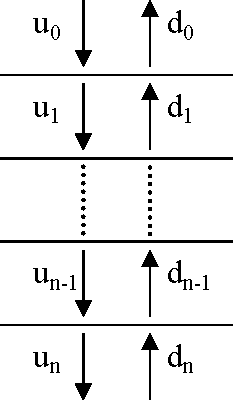
\includegraphics[width=0.25\textwidth]{figures/multilayer.pdf}
\caption{Schematic representation of the structure assumed by the scattering }
\end{figure}






\chapter{Reference Guide}
In this chapter a detailed explanation of the module is provided. For each sub-module a summary of the classes and function involved can be found, together with details on the most common functions.
\section{Module composition}
The A-FMM module in turn composed by different submodules:
\begin{itemize}
\item creator module: Contain the creator class, used to define the dielectric costant of the single layer.   
\item layer module: Contain the layer class, used to solve the Maxwell equation inside each single layer. It requires a creator instance to be initialized.
\item scattering module: Contain the S\_matrix class. All method for scattering matrix creation and manipulation are here implemented.  
\item satck module: Contain the stack class, used to calculate the Scattering Matrix and related quantities of the hole structure. It is initialize from a collection of layer instances.
\item sub\_sm module: Contains auxiliary function that are called in more than one module. It is non loaded by default when loading A\_FMM.
\end{itemize}

\section{Scattering module}
\subsection{S\_matrix class}
\subsubsection{Definition ad initialization}
This class contains the definition of the scattering matrix object and all method for scattering matrix manipulation. The scattering matrix is an object relating the amplitudes of the incoming end outgoing modes of a structure. It presets itself as following:
\begin{equation} \label{eq:S_matrix_def}
\left[
\begin{array}{c}
u' \\
d  \\
\end{array} 
 \right] = \left[
 \begin{array}{cc}
S_{11} & S_{12} \\
S_{21} & S_{22} \\
\end{array}
 \right]
 \left[
\begin{array}{c}
u \\
d' \\
\end{array} 
\right]
\end{equation}
following the convention of figure \ref{fig:SM_conv}.
\begin{figure}
\centering
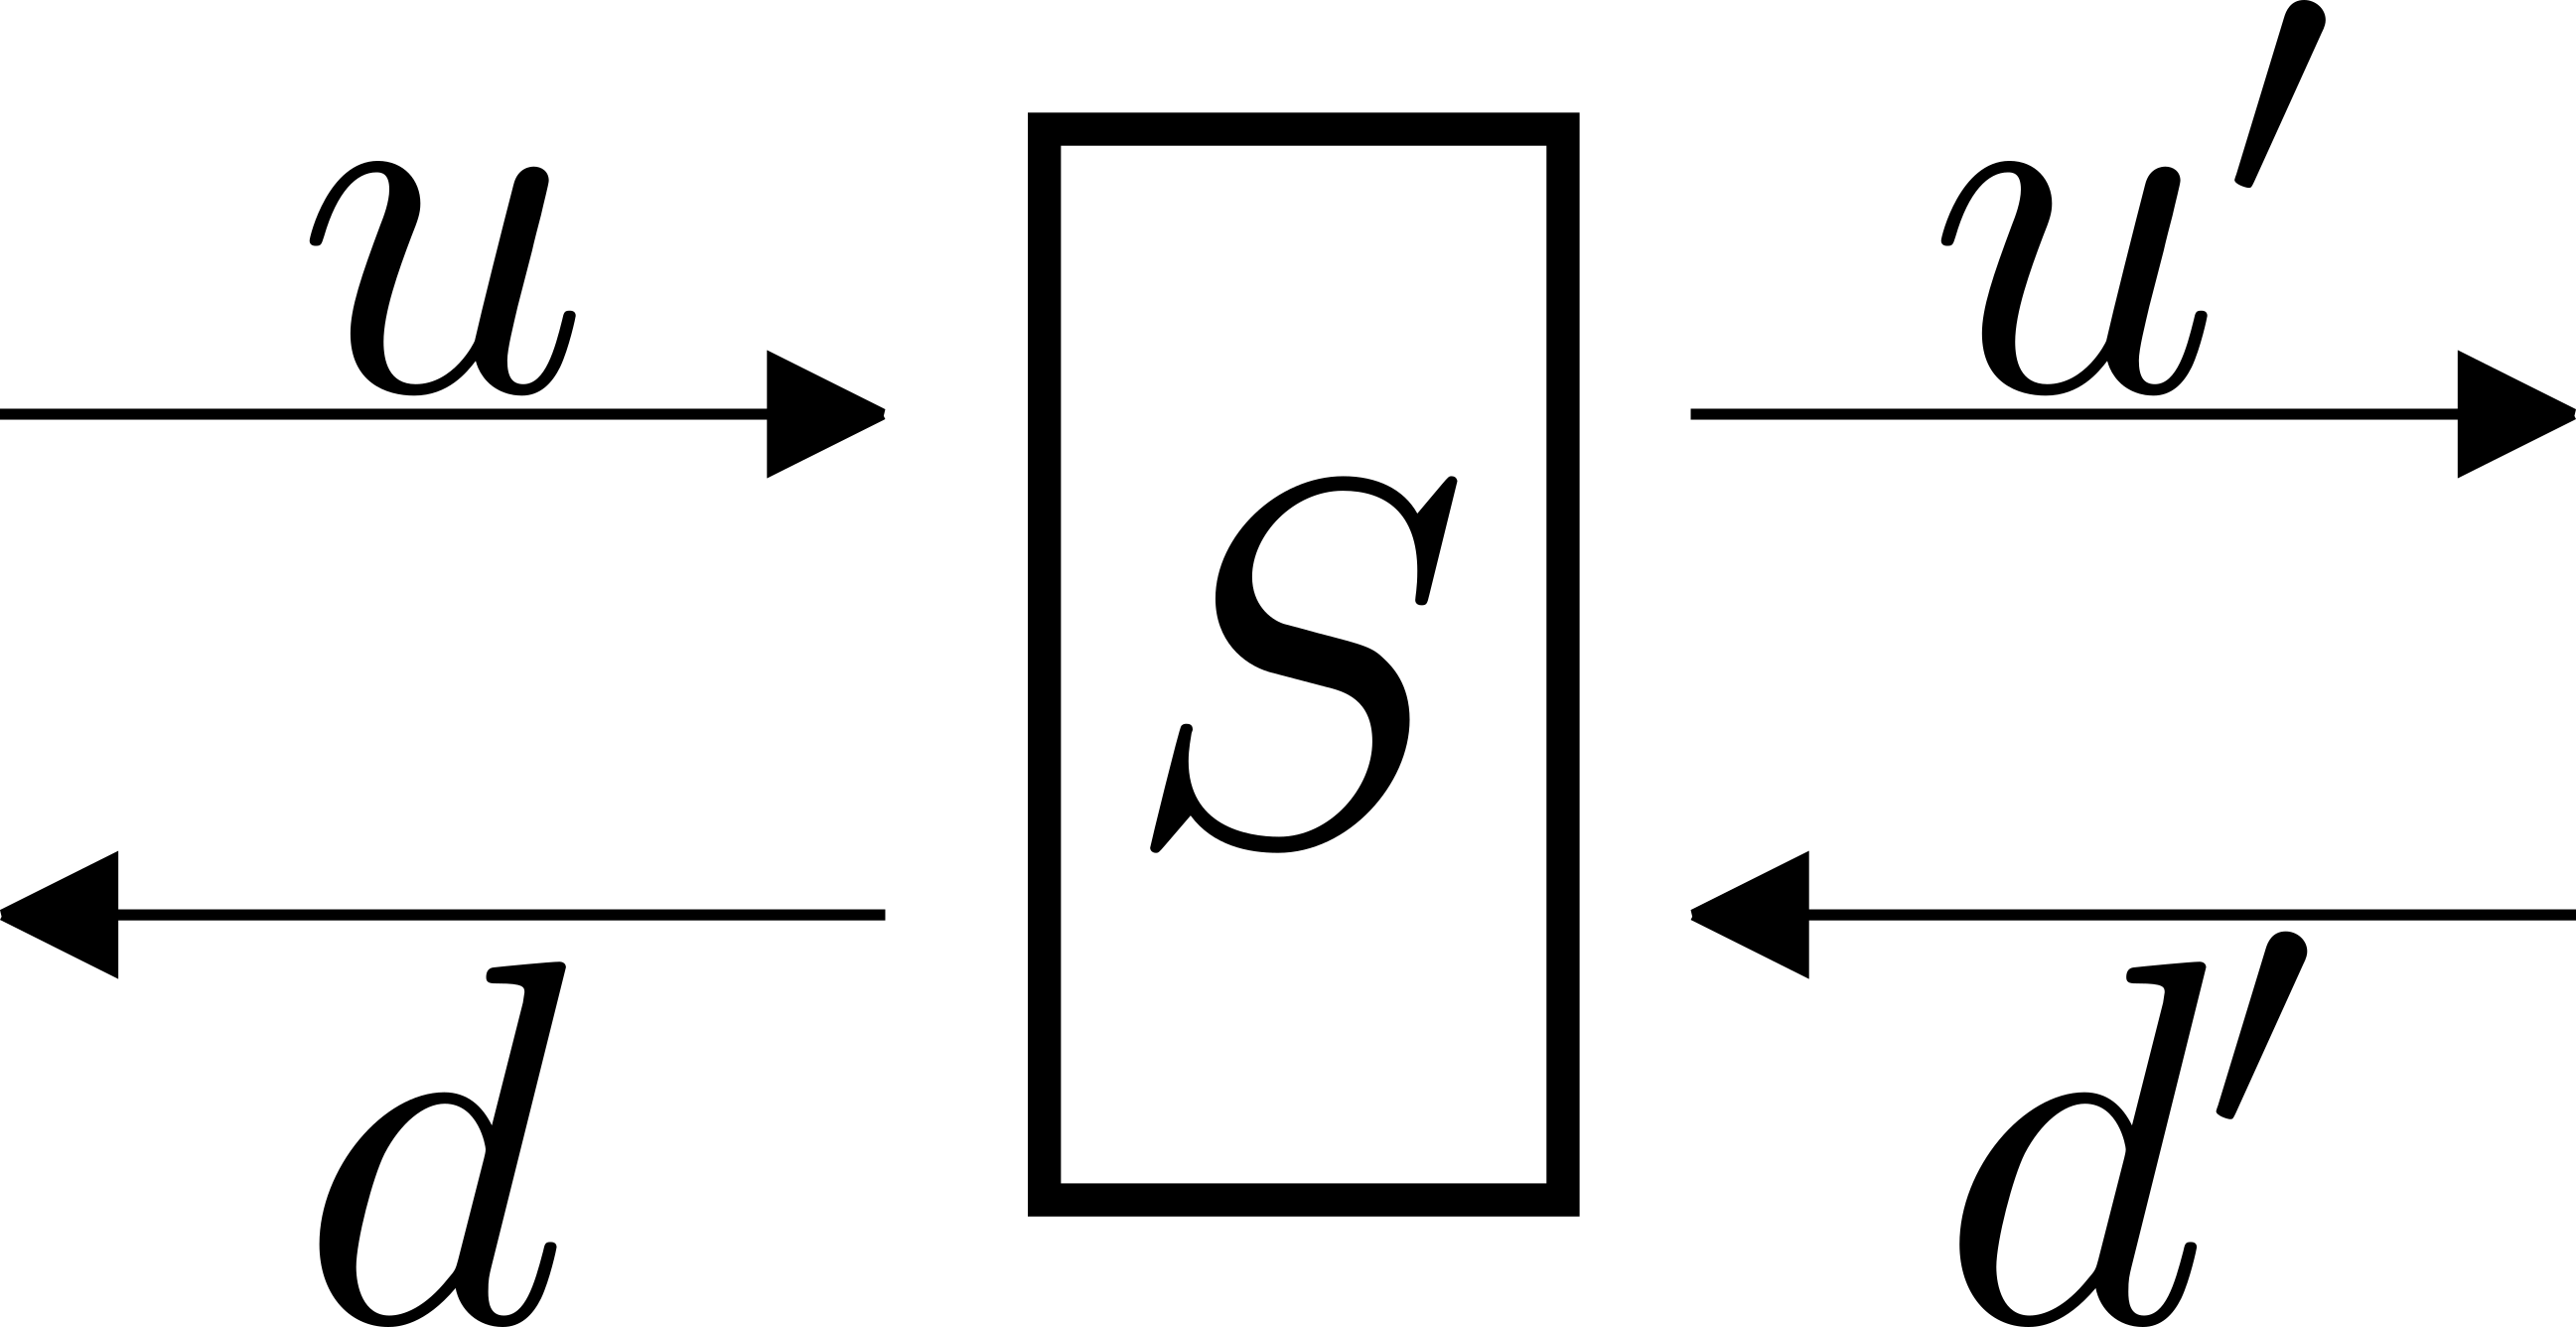
\includegraphics[width=0.5\textwidth]{figures/S.png}
\caption{Convention adopted for the scattering matrix formalism.} \label{fig:SM_conv}
\end{figure}
An instance is initialized as:
\begin{lstlisting}[language=Python]
S=S_matrix(N)
\end{lstlisting}
where \texttt{N} is the dimension of the four $N \times N$ matrices composing the scattering matrix. Each of this matrix is saved as an \texttt{numpy.ndarray} as an attribute of the S\_matrix object. For example to the $(1,2)$ element of the $S_{21}$ matrix is accessed as \texttt{S.S21[1,2]}.

\subsubsection{Method}
\begin{lstlisting}[language=Python,basicstyle=\ttfamily\Large]
add(s)
\end{lstlisting}
Takes as input an other instance of the S\_matrix class s, which is then joined to the right to the scattering matrix that calls the method.

\begin{lstlisting}[language=Python,basicstyle=\ttfamily\Large]
add_left(s)
\end{lstlisting}
Same as \texttt{add} but s matrix is joined to the left.

\begin{lstlisting}[language=Python,basicstyle=\ttfamily\Large]
add_uniform(lay,d)
\end{lstlisting}
Takes as input:
\begin{itemize}[noitemsep,topsep=0pt,parsep=0pt,partopsep=0pt]
\item \texttt{lay}: An instance of the layer class;
\item \texttt{d}: A float representing the thickness of the layer.
\end{itemize}
This method creates the scattering matrix for propagation trough a layer \texttt{lay} of thickness \texttt{d}, and then joins it to the right of the scattering matrix that calls the method.

\begin{lstlisting}[language=Python,basicstyle=\ttfamily\Large]
add_uniform_left(lay,d)
\end{lstlisting}
Same as \texttt{add\_uniform} but joins to the left.





\section{Layer Module}
\subsection{Layer class}
\subsubsection{Initialization}
This module contains several implementation of the layer class, which is responsable for definition of the single layer inside the scattering matrix approach. It also contains the methods for adding the coordinate transform an plotting of the mode fields. The different layer are:
\begin{lstlisting}[language=Python]
lay=layer(Nx,Ny,creator,Nyx=1.0)
\end{lstlisting}
which is the standard implementation of the class. A \texttt{creator} object is needed for the creation, and all the calculation for the Fourier transform are done analytically. The parameter for the initialization are:
\begin{itemize}[noitemsep,topsep=0pt,parsep=0pt,partopsep=0pt]
\item \texttt{Nx,Ny}: Trucation order respectively in $x$ and $y$ direction. Actual number of plane waves is $(2N_x+1)(2N_y+1)$.
\item \texttt{creator}: The creator instance describing the dielectric function.
\item \texttt{Nyx}: Ratio between the cell period in $y$ and $x$ direction (default is 1.0).
\end{itemize}

\begin{lstlisting}[language=Python]
lay=layer_num(Nx,Ny,func,args=(),Nyx=1.0,NX=1024,NY=1024)
\end{lstlisting}
Implementation in which the Fourier transforms for the layer are handled numerically. It is more versatile than the standard implementation, albeit should be less precise. The profile of the dielectric is obtained from the function \texttt{func}. The objects needed are:
\begin{itemize}[noitemsep,topsep=0pt,parsep=0pt,partopsep=0pt]
\item \texttt{Nx,Ny}: Integers, trucation order respectively in $x$ and $y$ direction. Actual number of plane waves is $(2N_x+1)(2N_y+1)$.
\item \texttt{func}: Function which defines the dielectric constant. It has to be in the form \texttt{func=func(x,y,..)}. After x and y additional parameters can be defined in the function and passed in \texttt{args}. Domain of the function in -0.5:0.5 in x and -0.5*Nyx:0.5*Nyx in y. 
\item \texttt{Nyx}: Ratio between the cell period in $y$ and $x$ direction (default is 1.0).
\item \texttt{args}: Tuple containing eventual additional parameters for \texttt{func}.
\item \texttt{NX,NY}: Integers, number of point in each direction used for numerical integration in the Fourier transforms.
\end{itemize}

\begin{lstlisting}[language=Python]
lay=layer_uniform(Nx,Ny,eps,Nyx=1.0)
\end{lstlisting}
Implementation of the uniform layer. It is implemented on is own because in this way its definition and solution are much faster. The parameters are:
\begin{itemize}[noitemsep,topsep=0pt,parsep=0pt,partopsep=0pt]
\item \texttt{Nx,Ny}: Trucation order respectively in $x$ and $y$ direction. Actual number of plane waves is $(2N_x+1)(2N_y+1)$.
\item \texttt{eps}: The dielectric constant of the uniform layer. Can be complex. 
\item \texttt{Nyx}: Ratio between the cell period in $y$ and $x$ direction (default is 1.0).
\end{itemize}
 


When initializing the layer class all the matrices involve in the eigenvalue problem for the layer are created.
\subsubsection{Methods}
\begin{lstlisting}[language=Python,basicstyle=\ttfamily\Large]
trasform(ex=0,ey=0)
\end{lstlisting}
Add the real coordinate transform.
\begin{itemize}[noitemsep,topsep=0pt,parsep=0pt,partopsep=0pt]
\item \texttt{ex,ey}: Respectively the width of the untransformed region in $x$ and $y$ direction. If not specified transformation in not applied in that direction.
\end{itemize}

\begin{lstlisting}[language=Python,basicstyle=\ttfamily\Large]
trasform_complex(ex=0,ey=0)
\end{lstlisting}
Add the complex coordinate transform simulating PML boundary conditions. 
\begin{itemize}[noitemsep,topsep=0pt,parsep=0pt,partopsep=0pt]
\item \texttt{ex,ey}: Respectively the width of the untransformed region in $x$ and $y$ direction. If not specified transformation in not applied in that direction.
\end{itemize}

\begin{lstlisting}[language=Python,basicstyle=\ttfamily\Large]
mode(k0,kx=0.0,ky=0.0,v=1)
\end{lstlisting}
Solve the eigenvalue problem of the layer.
\begin{itemize}[noitemsep,topsep=0pt,parsep=0pt,partopsep=0pt]
\item \texttt{k0}: Energy of the mode
\item \texttt{kx,ky}: Respectively the lateral wavevector in the $x$ and $y$ direction (in unit of inverse of the period).
\item  \texttt{v}: If equal to 0 only eigenvalue are calculated. Useful when interested only in propagation constant of the mode of the single layer. Default is 1.
\end{itemize}
create three new attributes of the class layer:
\begin{itemize}[noitemsep,topsep=0pt,parsep=0pt,partopsep=0pt]
\item \texttt{W}: Vector of the eigenvalues (effective indexes of modes squared). 
\item \texttt{V}: Matrix of electric eigenvectors of the modes. \texttt{V[:,i]} is the vector to the $i^{th}$ mode.
\item \texttt{VH}: Matrix of magnetic eigenvectors of the modes. Same convention as \texttt{V}.
\end{itemize}

\begin{lstlisting}[language=Python,basicstyle=\ttfamily\Large]
eps_plot(pdf=None,N=200,s=1.0)
\end{lstlisting}
Plot dielectric function profile reconstructed from fourier transform.
\begin{itemize}[noitemsep,topsep=0pt,parsep=0pt,partopsep=0pt]
\item \texttt{pdf}: Name of the pdf file used to save the figure (string, without the .pdf).
\item \texttt{N}: Width in pixel of the cell. Default 200.
\item \texttt{s}: Number of fundamental cells plotted. Default 1.
\end{itemize}

\begin{lstlisting}[language=Python,basicstyle=\ttfamily\Large]
plot_E(pdf,i,N=100,s=1,func=np.abs)
\end{lstlisting}
Plot electric field profile of selected mode.
\begin{itemize}[noitemsep,topsep=0pt,parsep=0pt,partopsep=0pt]
\item \texttt{pdf} Instances of the PdfPages class. Specify pdf file where to save field.
\item \texttt{i} Number of mode to plot. Mode are ordered in decreasing effective index. Numeration start at 1.
\item \texttt{N} Width in pixel of the cell. Default 100.
\item \texttt{s} Number of fundamental cells plotted. Default 1.
\item \texttt{func} Since field is complex, function to apply to field before plotting. Default is abs. Useful can be real, imag, angle. 
\end{itemize}

\begin{lstlisting}[language=Python,basicstyle=\ttfamily\Large]
plot_H(pdf,i,N=100,s=1,func=np.abs)
\end{lstlisting}
Plot magnetic field profile of selected mode. Same inputs as \texttt{plot\_E}.

\begin{lstlisting}[language=Python,basicstyle=\ttfamily\Large]
plot_field(pdf,i,N=100,s=1,func=np.abs)
\end{lstlisting}
Plot both electric and magnetic field profile of selected mode. Same inputs as \texttt{plot\_E}. 

\begin{lstlisting}[language=Python,basicstyle=\ttfamily\Large]
get_field(x,y,i,func=np.abs)
\end{lstlisting}
Return field of selected mode at selected point. 
\begin{itemize}[noitemsep,topsep=0pt,parsep=0pt,partopsep=0pt]
\item \texttt{x,y} Coordinate of the point in which to calculate fields.
\item \texttt{i} Number of mode to plot. Mode are ordered in decreasing effective index. Numeration start at 1.
\item \texttt{func} Since field is complex, function to apply to field before plotting. Default is abs. Useful can be real, imag, angle. 
\end{itemize}
Return 1-dim array of length 4 containing in order: Ex,Ey,Hx,Hy

\begin{lstlisting}[language=Python,basicstyle=\ttfamily\Large]
get_P_norm()
\end{lstlisting}
Calculate z component of Poynting vector, used in the scattering matrix algorithm to normalize correctly reflection ad transmission.
The values of Poynting vector are then stored in the new attribute \texttt{P\_norm}.

\begin{lstlisting}[language=Python,basicstyle=\ttfamily\Large]
T_interface(lay)
\end{lstlisting}
Takes in input a different instance of the layer class. Return the transfer matrix representing the interface between the layer that calls the method and the layer given ad input.  The obtained matrix is an instance of \texttt{numpy.ndarray}. 

\begin{lstlisting}[language=Python,basicstyle=\ttfamily\Large]
T_prop(d)
\end{lstlisting}
Takes in input a float value \texttt{d} representing the thickness of the layer. Return the transfer matrix of the propagation trough a thickness d of the layer that calls the method. Could generate numerical instabilities.  The obtained matrix is an instance of \texttt{numpy.ndarray}. 

\begin{lstlisting}[language=Python,basicstyle=\ttfamily\Large]
interface(lay)
\end{lstlisting}
Takes in input a different instance of the layer class. Return the scattering matrix representing the interface between the layer that calls the method and the layer given ad input.  The obtained matrix is an instance of \texttt{S\_matrix}. 




\end{document}
\begin{lstlisting}[language=Python,basicstyle=\ttfamily\Large]
\end{lstlisting}
\begin{itemize}[noitemsep,topsep=0pt,parsep=0pt,partopsep=0pt]
\item \texttt{Nx,Ny}
\end{itemize}
